\section{Timed Rebeca and Floating Time Transition System} \label{sec::FTTS}

Timed Rebeca is an extension of Rebeca where we can model computational time, network delays, and periodic events \cite{Arni}.

Floating Time Transition System (FTTS) is proposed based on the isolation of timed rebecs \cite{FACS2015,SCP}. The idea behind FTTS is similar to partial order reduction (POR) but the technique does not fit exactly in the definition of POR. What we mean by floating time is that in each state of the state space, different actors do not necessarily have the same local clock, i.e.,  actors are not synchronised on their local time in the state space. We consider this as letting the time \textit{float} across the actors in the state space. 
To avoid confusion, it is important to note the different models in different levels of abstraction, and also layering of models. We have (1) distributed systems, we use (2) Timed Rebeca to model distributed systems, and we model (3) the state space as Floating Time Transition System to do the analysis. 
%
Note that at the level of Timed Rebeca, actors have synchronised local clocks which gives us a notion of global time across the model. We use time stamps, and time stamps are comparable across all actors in the model. This makes our model simpler and more understandable, and our analysis more efficient.
But in distributed systems we cannot assume synchronised clocks and time stamps. 
For that assumption to be valid and faithful enough to the system,  we rely on the layering and different responsibilities for different layers. For distributed actors (as faithful representatives of distributed software components) to be able to have synchronised clocks and comparable time stamps we rely on the lower-level network protocols to provide that for us. 

In Timed Rebeca we have a concept of time and we can consider that each statement is executed at a certain point in time. Note that we are now talking at the level of the Rebeca model, the notion of time is the model time, and we do not need to worry about synchronising the clocks among different components in the distributed system. We assume that local clocks of actors are synchronised and we can have comparable time stamps on each statement in the actors.
%
In Timed Rebeca models, we use a \texttt{delay(t)} statement to show the computation delay. Other statements are assumed to be executed in zero time. We use  \texttt{after(t)} in combination with a \texttt{send} message statement, it means that the time stamp of the message when it is put in the queue of the receiver is the value of the local clock of the sender (\texttt{now} in the sender) plus the value of \texttt{t}.
The progress of time is forced by the \texttt{delay} statement and also by \texttt{after}. 
We can assume that the time stamp of all the statements are zero when a model starts to execute, then in each actor the local time is increased by value of \texttt{t} if there is a \texttt{delay(t)} statement.
A \texttt{send} statement with an  \texttt{after} does not cause any increase in the local time per se. The statement following the \texttt{send} statement has the same time stamp as the \texttt{send} statement itself.
The \texttt{after} construct may cause an increase in the time when the actor picks the message annotated by \texttt{after} to be executed. The local time of the receiver actor is set to the time stamp of the message, unless it is already greater than that.
The latter situation means that the message has been sitting in the queue while the actor has been busy executing another message.
Remember that messages are executed atomically and are not preempted.
%
The progress of time happens in the case that the time stamp of the message is greater than the local time of the receiver actor, the local time will be pushed forward.
%
The \texttt{after} construct can be used to model the network delay, and also to model periodic events.


If we use the standard Timed Transition System (TTS) to generate the state space for Timed Rebeca model we distinguish three types of transitions: $\tau$ transitions, \textit{events}, and \textit{timed} transitions.
In FTTS we reduce that to only \textit{events} transitions.
%
We explain TTS and FTTS for Timed Rebeca using an example in Listing \ref{src::FTTS-actor-model}.
Listing \ref{src::FTTS-actor-model} shows a simple Rebeca model with two rebecs $r1$ and $r2$ instantiated from two reactive classes $RC1$ and $RC2$.
$RC1$ has only one message server ($m1$) in which it triggers the two message servers of $RC2$ ($m2$ and $m3$).
The two message servers of $RC2$ are event handlers that do nothing, i.e., there are no internal actions caused by statements like assignments, or \texttt{send}, and no  \texttt{delay} statements. Note that \texttt{send} statements are considered as internal or silent actions but they cause a change in the message queue of the receiver by adding the sent message to that queue.
 

Figure \ref{fig::FTTSandTTS}.a shows the TTS generated for the model in Listing \ref{src::FTTS-actor-model}. 
The constructor of $RC1$ puts the message $m1$ in the queue of $RC1$. So, in $time=0$ we have the message $m1$ in the queue of $r1$ (see state $s_0$ in Figure \ref{fig::FTTSandTTS}.a). Also, you see that the message queue of $r2$ is empty. On the transition from $s_0$ to $s–1$ the message is taken from the queue of $r–1$, and in the state $s_1$ the method $m_1$ is ready to be executed, i.e., the Program Counter (PC) is at $m1:1$. The first statement in $m_1$ is a \texttt{delay} statement which is executed and pushes the time forward to $time=2$ in state $s_2$.
In the state $s_2$, the PC points at a $send$ statement: $r_2.m_2()$. After this statement is executed as a silent or $\tau$ statement, we have the message $(r_1 \rightarrow r_2.m_2(), 0, \infty)$ in the queue of $r–2$


\begin{lstlisting}[language=rebeca, caption= A simple Timed Rebeca model with two rebecs, label=src::FTTS-actor-model]
reactiveclass RC1 (3) {
	knownrebecs {
		RC2 r2;
	}
	RC1() {
		self.m1();
	}
	msgsrv m1() {
		delay(2); %PC = 1
		r2.m2();  %PC = 2 
		delay(2); %PC = 3 
		r2.m3();  %PC = 4
		self.m1() after (10); %PC = 5
	}
}
reactiveclass RC2 (4) {
	knownrebecs {
		RC1 r1;
	}
	RC2() { }
	msgsrv m2() { }
	
	msgsrv m3() { }
}

main {
	RC1 r1(r2):();
	RC2 r2(r1):();
}

\end{lstlisting}

\begin{figure}
\centering
\begin{subfigure}[b]{0.2\textwidth}
%\subfigure[TTS]{
%\label{fig::TTS}
  \centering
  \small{
   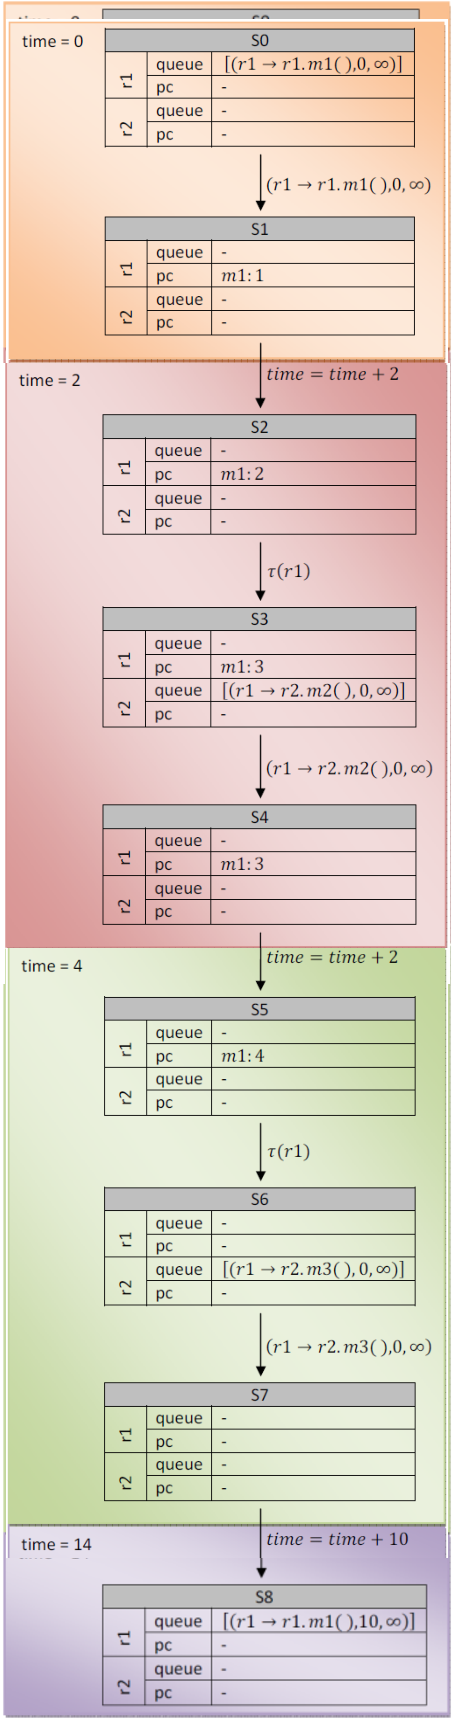
\includegraphics[width=.8\textwidth]{TTSCorrect.pdf}
  }
  \caption{TTS}
  \label{fig::TTS}
%}
\end{subfigure}
%\qquad
\begin{subfigure}[b]{0.2\textwidth}
%\subfigure[FTTS]{
%\label{fig::FTTS}
  \centering
  \small{
   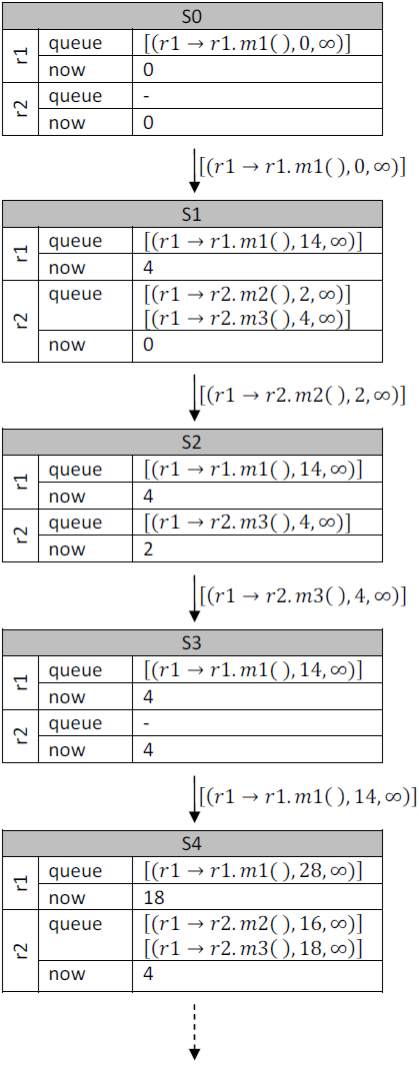
\includegraphics[width=.8\textwidth]{Picture2-FTTS.pdf}
   \caption{FTTS}
   \label{fig::FTTS}
  }
%}
\end{subfigure}
\caption{ TTS and FTTS for the Timed Rebeca model in Listing \ref{src::FTTS-actor-model}.}
\label{fig::clinger-cdg}
\end{figure}

\begin{figure}
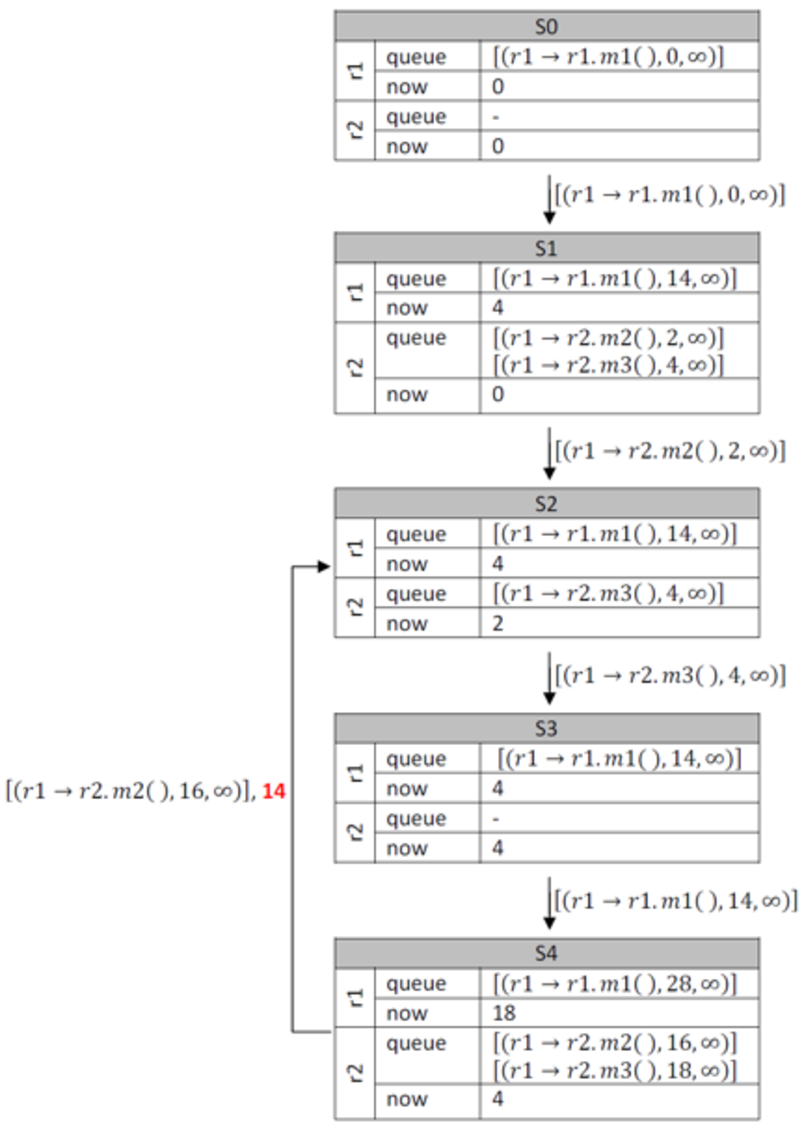
\includegraphics[width=.35\textwidth]{Picture3-BFTTS.pdf}
\caption{ Bounded FTTS for the Timed Rebeca model in Listing \ref{src::FTTS-actor-model}.}
\label{fig::FTTSandTTS}
\end{figure}
